\documentclass{beamer}
%\usetheme{Boadilla}
%\usetheme{Szeged}
%\usetheme{Singapore}
%\usetheme{Frankfurt}
\usecolortheme{dove}
%\setbeamertemplate{navigation symbols}{{\footnotesize\insertframenumber}}
\setbeamertemplate{navigation symbols}{}
%\setbeamertemplate{headline}{%
  %  \leavevmode%
    %\hbox{%
    %\insertsectionnavigationhorizontal{\textwidth}{\hspace{20pt}}{\hspace{20pt}}
  %}
%}
\newenvironment{alltt}{\ttfamily}{\par}
\usepackage{amsmath,amssymb,amsfonts,amsthm, multicol, subfigure, color}
\usepackage{bm}
\usepackage{graphicx}
\usepackage{tabularx}
\usepackage{booktabs}
\usepackage{hyperref}
\usepackage{pdfpages}
\usepackage{xcolor}
\definecolor{dodgerblue}{rgb}{.118, .575, 1}
\definecolor{seagreen4}{RGB}{46, 139, 87}
\def\independenT#1#2{\mathrel{\rlap{$#1#2$}\mkern2mu{#1#2}}}
\newcommand\independent{\protect\mathpalette{\protect\independenT}{\perp}}
\newcommand\indep{\protect\mathpalette{\protect\independenT}{\perp}}
\def\logit{\text{logit}}
\usepackage{stackrel}
\usepackage{tikz}
\usetikzlibrary{arrows,shapes.arrows,positioning,shapes,patterns,calc}
\newcommand\slideref[1]{\vskip .1cm \scriptsize \textcolor{gray}{{#1}}}
\newcommand\red[1]{{\color{red}#1}}
\newcommand\bred[1]{{\color{red}\textbf{#1}}}
\newcommand\blue[1]{{\color{blue}#1}}
\newcommand\bblue[1]{{\color{blue}\textbf{#1}}}
\newcommand\gray[1]{{\color{gray}#1}}
\newcommand\bgray[1]{{\color{gray}\textbf{#1}}}
\newcommand\green[1]{{\color{seagreen4}#1}}
\newcommand\bgreen[1]{{\color{seagreen4}\textbf{#1}}}
\newcommand\purple[1]{{\color{purple}#1}}
\newcommand\orange[1]{{\color{orange}#1}}
\newcommand\black[1]{{\color{black}#1}}
\newcommand\white[1]{{\color{white}#1}}
\newcommand\teal[1]{{\color{teal}#1}}
\newcommand\magenta[1]{{\color{magenta}#1}}
\newcommand\Fuchsia[1]{{\color{Fuchsia}#1}}
\newcommand\BlueGreen[1]{{\color{BlueGreen}#1}}
\colorlet{lightgray}{gray!40}
\pgfdeclarelayer{bg}    % declare background layer for tikz
\pgfsetlayers{bg,main} % order layers for tikz
\newcommand\mycite[1]{\begin{scriptsize}\textcolor{darkgray}{(#1)}\end{scriptsize}}
\newcommand\iid{\stackrel{\text{iid}}{\sim}}
\newcommand\E{\text{E}}
\newcommand\V{\text{V}}
\renewcommand\P{\text{P}}
\newcommand{\Cov}{\text{Cov}}
\newcommand{\Cor}{\text{Cor}}
\newcommand\doop{\text{do}}
\newcommand{\tcframe}{\frame{
\small{
\only<1|handout:0>{\tableofcontents}
\only<2|handout:1>{\tableofcontents[currentsection]}}
}}
% Credit for the following to https://tex.stackexchange.com/questions/44983/beamer-removing-headline-and-its-space-on-a-single-frame-for-plan-but-keepin
\makeatletter
    \newenvironment{withoutheadline}{
        \setbeamertemplate{headline}[default]
        \def\beamer@entrycode{\vspace*{-\headheight}}
    }{}
\makeatother
\setbeamercovered{invisible}
\usepackage[round]{natbib}
\bibliographystyle{humannat-mod}
\setbeamertemplate{enumerate items}[default]
\usepackage{mathtools}
% BELOW THREE LINES MAKES NAME IN FOOTER
\setbeamertemplate{footline}[text line]{%
%\parbox{\linewidth}{\vspace*{-8pt}Ian Lundberg (Princeton)}}
\parbox{\linewidth}{\vspace*{-8pt}\bgray{Ian Lundberg (UCLA)}\hfill
\insertsectionnavigationhorizontal{.7\paperwidth}{}{\hfill\hfill}}
}
%\hfill \insertframenumber/23}}%\hfill\insertshortauthor\hfill\insertpagenumber}}
%\setbeamertemplate{navigation symbols}{}
\usepackage{framed}
\usepackage{soul}
\usepackage{appendixnumberbeamer}

\title{Quantifying the contribution of occupational segregation to racial disparities in health: A gap-closing perspective}
\author{Ian Lundberg}
\date{UCLA\\8 August 2020}

\begin{document}

{
%\setbeamertemplate{footline}[text line]{\parbox{\linewidth}{\vspace*{-8pt}Ian Lundberg (UCLA)\hfill}}
\begin{frame}
\begin{tikzpicture}[x = \textwidth, y = \textheight]
\node at (0,0) {};
\node at (1,1) {};
\node[anchor = north west, align = left, font = \LARGE] at (0,.9) {Quantifying the Contribution of\\Occupational Segregation to\\Racial Disparities in Health};
\node[anchor = north west, align = left, font = \Large] at (0,.63) {A Gap-Closing Perspective};
% At top right
%\node[anchor = north east, align = right, font = \Large] at (1,.6) {\bgray{Ian Lundberg}};
%\node[anchor = north east, align = right, font = \footnotesize] at (1,.5) {Princeton University\\Department of Sociology\\ilundberg@princeton.edu};
% At bottom left
\node[anchor = north, align = center, font = \Large] at (.5,.47) {\bgray{Ian Lundberg}};
\node[anchor = south, align = center, font = \footnotesize] at (.5,.27) {University of California, Los Angeles\\ianlundberg@ucla.edu};
\node[anchor = south west, align = left, font = \tiny, text width = \textwidth] at (0,.1) {Research reported in this publication was supported by the National Science Foundation under Award Number 2104607 and by the Eunice Kennedy Shriver National Institute of Child Health \& Human Development of the National Institutes of Health under Award Number P2CHD047879 and P2CHD041022.\\Replication code is available at github.com/ilundberg/replication};
\end{tikzpicture}
\end{frame}

\section{A Disparity}

% SCATTERPLOT
\begin{frame}
\label{descriptive_results}
\begin{tikzpicture}[x = \textwidth, y = \textheight]
\node at (0,0) {};
\node at (1,1) {};
\node<1->[anchor = north east, font = \footnotesize, align = right, gray] (note1) at (1,.65) {Current\\Population Survey\\Annual Social and\\Economic Supplement\\Ages 25--60\\2005--2020};
\node<2->[anchor = north east, font = \footnotesize] at (.33,.95) {Race};
\node<2->[anchor = north east, font = \footnotesize] at (.33,.81) {Work-Limiting Disability};
\node<3>[anchor = north west] at (0,.7) {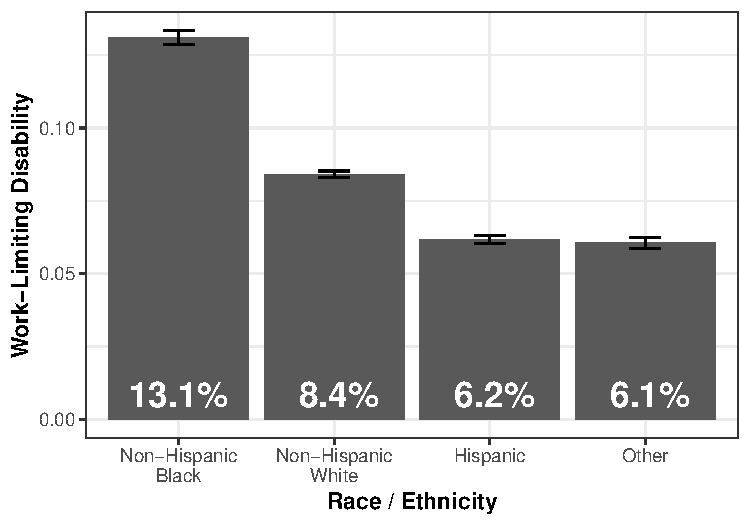
\includegraphics[width = .68\textwidth]{figures/disability_by_race}};
\node<4->[anchor = north east, font = \footnotesize] at (.33,.88) {Occupation};
\node<5->[anchor = north west, font = \footnotesize] at (.35,.95) {(reported at year 1)};
\node<5->[anchor = north west, font = \footnotesize] at (.35,.88) {(reported at year 1)};
\node<6->[anchor = north west, font = \footnotesize] at (.35,.81) {(reported at year 2)};
\node<7>[anchor = north west] at (0,.7) {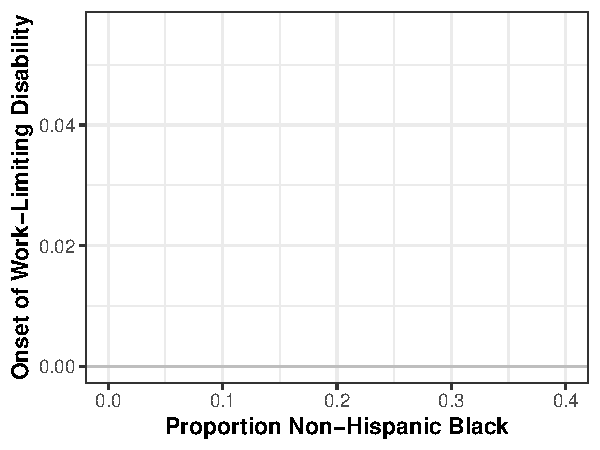
\includegraphics[width = .68\textwidth]{figures/scatter_factual_outcome_re_NonHispanicBlack_slide1}};
\node<8>[anchor = north west] at (0,.7) {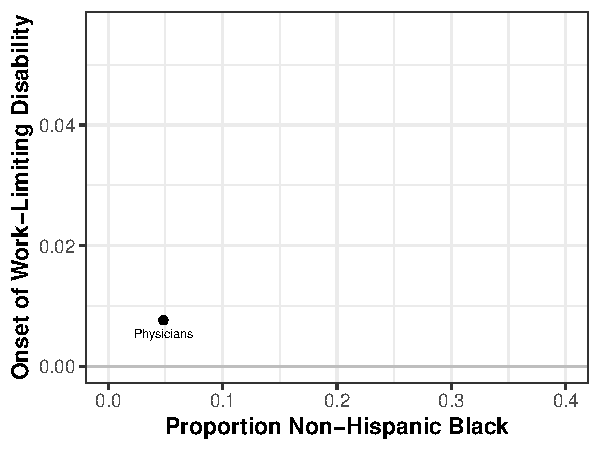
\includegraphics[width = .68\textwidth]{figures/scatter_factual_outcome_re_NonHispanicBlack_slide2}};
\node<9>[anchor = north west] at (0,.7) {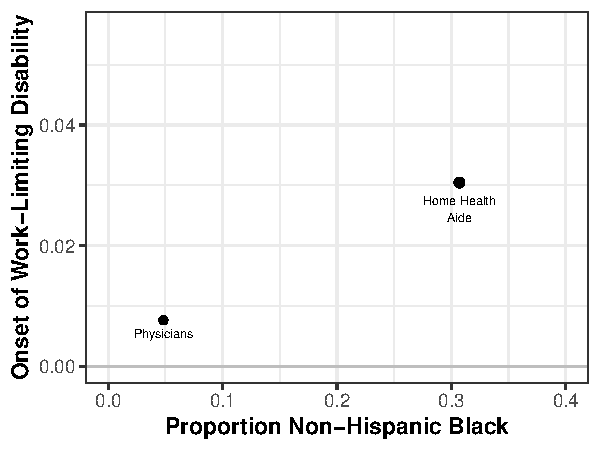
\includegraphics[width = .68\textwidth]{figures/scatter_factual_outcome_re_NonHispanicBlack_slide3}};
\node<10>[anchor = north west] at (0,.7) {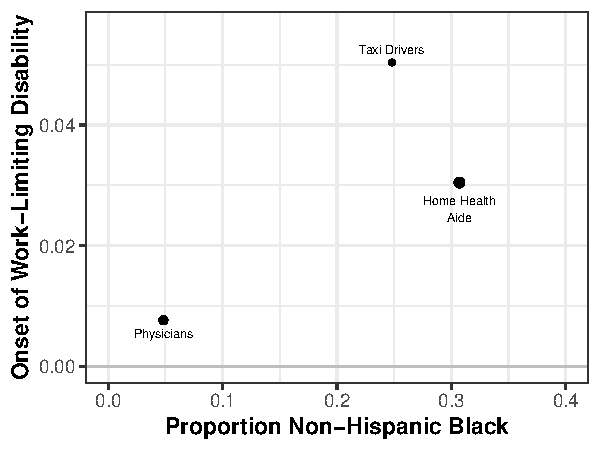
\includegraphics[width = .68\textwidth]{figures/scatter_factual_outcome_re_NonHispanicBlack_slide4}};
\node<11>[anchor = north west] at (0,.7) {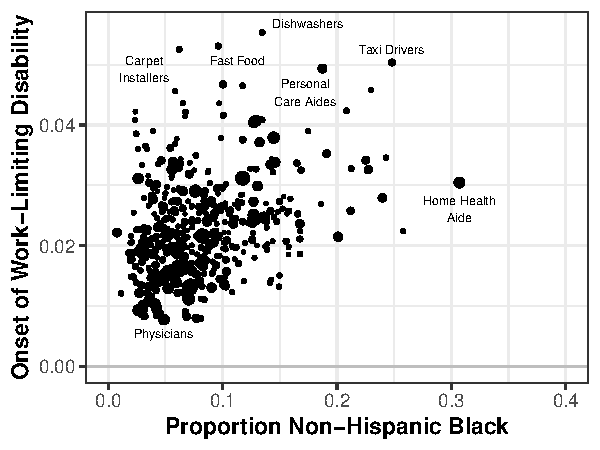
\includegraphics[width = .68\textwidth]{figures/scatter_factual_outcome_re_NonHispanicBlack_slide5}};
\node<12>[anchor = north west] at (0,.7) {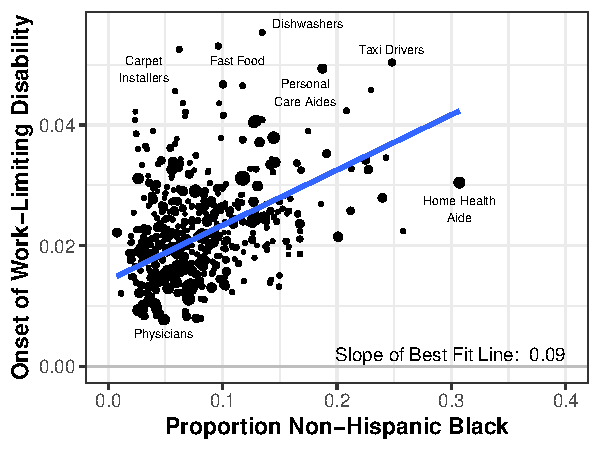
\includegraphics[width = .68\textwidth]{figures/scatter_factual_outcome_re_NonHispanicBlack_slide6}};
\end{tikzpicture}
\end{frame}

\section{A Counterfactual Setting}

% ASA SIMLIFIED METHODS BIT
% Plan is:
% 1. Contribution
% 2. Table
% 3. Each person has an occupation
% 4. Each person has a health outcome
% 5. Person 1 counterfactual home health aid (question mark)
% 6. Question marks for all potential outcomes
% 7. Counterfactuals disappear
% 8. Begin prediction sequence
% Next slide: Conditions for this to work
\begin{frame}
\begin{tikzpicture}[x = \textwidth, y = \textheight]
\node at (0,0) {};
\node at (1,1) {};
% SLIDE 1: Contribution
%\node[anchor = north] (how) at (.5, .95) {Quantifying the \bblue{contribution} of occupation};
\node[anchor = north] (how) at (.5, .95) {\bgray{A Counterfactual Setting:} Eliminate occupational segregation};
\draw[line width = 2pt, gray, line cap = round] (how.south west) -- (how.south east);
% SLIDE 2: Set up the table
\only<2->{
\node[anchor = south, font = \footnotesize, rotate = 90] at (.05, .375) {\bgray{White}};
\node[anchor = south, font = \footnotesize, rotate = 90] at (0.05, .175) {\bgray{Black}};
\node[anchor = east, font = \footnotesize] at (.2, .45) {Person 1};
\node[anchor = east, font = \footnotesize] at (.2, .4) {Person 2};
\node[anchor = east, font = \footnotesize] at (.2, .35) {Person 3};
\node[anchor = east, font = \footnotesize] at (.2, .3) {Person 4};
\draw[thick, dashed] (.05,.275) -- (.75,.275);
\node[anchor = east, font = \footnotesize] at (.2, .25) {Person 5};
\node[anchor = east, font = \footnotesize] at (.2, .2) {Person 6};
\node[anchor = east, font = \footnotesize] at (.2, .15) {Person 7};
\node[anchor = east, font = \footnotesize] at (.2, .1) {Person 8};
\node[anchor = south, font = \footnotesize, align = center] at (.3, .5) {Administrative\\Assistant};
\node[anchor = south, font = \footnotesize, align = center] at (.5, .5) {Home Health\\Aid};
\node[anchor = south, font = \footnotesize, align = center] at (.7, .5) {Sales\\Supervisor};
}
% SLIDE 3: Each person has one cell
\only<3->{
\node[draw, line width = .5pt, circle, fill = lightgray, fill opacity = 1, inner sep = 3pt] (1a) at (.3, .45) {};
\node[draw, line width = .5pt, circle, fill = lightgray, fill opacity = 1, inner sep = 3pt] (2a) at (.3, .4) {};
\node[draw, line width = .5pt, circle, fill = lightgray, fill opacity = 1, inner sep = 3pt] (3b) at (.5, .35) {};
\node[draw, line width = .5pt, circle, fill = lightgray, fill opacity = 1, inner sep = 3pt] (4c) at (.7, .3) {};
\node[draw, line width = .5pt, diamond, fill = lightgray, fill opacity = 1, inner sep = 3pt] (5b) at (.5, .25) {};
\node[draw, line width = .5pt, diamond, fill = lightgray, fill opacity = 1, inner sep = 3pt] (6c) at (.7, .2) {};
\node[draw, line width = .5pt, diamond, fill = lightgray, fill opacity = 1, inner sep = 3pt] (7b) at (.5, .15) {};
\node[draw, line width = .5pt, diamond, fill = lightgray, fill opacity = 1, inner sep = 3pt] (8a) at (.3, .1) {};
}
% SLIDE 4: Health outcomes
\only<4-10>{
\node[font = \scriptsize] at (1a) {\textcolor{seagreen4}{$\checkmark$}};
\node[font = \scriptsize] at (2a) {\textcolor{seagreen4}{$\checkmark$}};
\node at (8a) {
\includegraphics[width = 7pt]{figures/injury}};
}
\only<4-11>{
\node at (3b) {
\includegraphics[width = 7pt]{figures/injury}};
\node at (5b) {
\includegraphics[width = 7pt]{figures/injury}};
\node at (7b) {
\includegraphics[width = 7pt]{figures/injury}};
}
\only<4-12>{
\node[font = \scriptsize] at (4c) {\textcolor{seagreen4}{$\checkmark$}};
\node[font = \scriptsize] at (6c) {\textcolor{seagreen4}{$\checkmark$}};
}
% SLIDE 5: One counterfactual
\only<5-6>{
\node[circle, fill = lightgray, fill opacity = 1, inner sep = 3pt] (1b) at (.5, .45) {};
}
\only<5-6>{
\node[font = \tiny] at (1b) {?};
}
% SLIDE 6: All counterfactuals
\only<6>{
\node[circle, fill = lightgray, fill opacity = 1, inner sep = 3pt] (3a) at (.3, .35) {};
\node[circle, fill = lightgray, fill opacity = 1, inner sep = 3pt] (4a) at (.3, .3) {};
\node[diamond, fill = lightgray, fill opacity = 1, inner sep = 3pt] (5a) at (.3, .25) {};
\node[diamond, fill = lightgray, fill opacity = 1, inner sep = 3pt] (6a) at (.3, .2) {};
\node[diamond, fill = lightgray, fill opacity = 1, inner sep = 3pt] (7a) at (.3, .15) {};
\node[circle, fill = lightgray, fill opacity = 1, inner sep = 3pt] (2b) at (.5, .4) {};
\node[circle, fill = lightgray, fill opacity = 1, inner sep = 3pt] (4b) at (.5, .3) {};
\node[diamond, fill = lightgray, fill opacity = 1, inner sep = 3pt] (6b) at (.5, .2) {};
\node[diamond, fill = lightgray, fill opacity = 1, inner sep = 3pt] (8b) at (.5, .1) {};
\node[circle, fill = lightgray, fill opacity = 1, inner sep = 3pt] (1c) at (.7, .45) {};
\node[circle, fill = lightgray, fill opacity = 1, inner sep = 3pt] (2c) at (.7, .4) {};
\node[circle, fill = lightgray, fill opacity = 1, inner sep = 3pt] (3c) at (.7, .35) {};
\node[diamond, fill = lightgray, fill opacity = 1, inner sep = 3pt] (5c) at (.7, .25) {};
\node[diamond, fill = lightgray, fill opacity = 1, inner sep = 3pt] (7c) at (.7, .15) {};
\node[diamond, fill = lightgray, fill opacity = 1, inner sep = 3pt] (8c) at (.7, .1) {};
}
\only<6>{
\node[font = \tiny] at (1c) {?};
\node[font = \tiny] at (2b) {?};
\node[font = \tiny] at (2c) {?};
\node[font = \tiny] at (3a) {?};
\node[font = \tiny] at (3c) {?};
\node[font = \tiny] at (4a) {?};
\node[font = \tiny] at (4b) {?};
\node[font = \tiny] at (5a) {?};
\node[font = \tiny] at (5c) {?};
\node[font = \tiny] at (6a) {?};
\node[font = \tiny] at (6b) {?};
\node[font = \tiny] at (7a) {?};
\node[font = \tiny] at (7c) {?};
\node[font = \tiny] at (8b) {?};
\node[font = \tiny] at (8c) {?};
}
% SLIDE 7: All counterfactuals disappear
% SLIDE 8: Begin prediction function
\node<8->[anchor = south] (input) at (.2,.78) {Input};
\draw<8->[thick] (input.south west) -- (input.south east);
\node<8->[font = \footnotesize, align = center, anchor = north] at (.2,.78) {$\text{Covariates}_i$\\$\text{Occupation}_i$};
%\node<8-11>[font = \footnotesize, align = center, anchor = north] at (.2,.78) {$\text{Covariates}_i$\\$\substack{\texttt{Administrative}\\\texttt{Assistant}}$};
\node<9->[draw = gray, line width = 1.2pt, rounded corners, align = center] at (.5,.73) {Prediction\\Function};
\draw<9->[->, thick] (.3,.73) -- (.37,.73);
\node<10->[anchor = south] (output) at (.8,.78) {Output};
\draw<10->[thick] (output.south west) -- (output.south east);
%\node<8-9>[font = \footnotesize, align = center, anchor = west] at (predicted.east) {$\left(\substack{\text{as an}\\\texttt{Administrative}\\\texttt{Assistant}}\right)$};
\node<10->[font = \footnotesize, align = center] (predicted) at (.8,.73) {$\hat{y}$};
\draw<10->[->, thick] (.63,.73) -- (.7,.73);
\only<11->{
\node[font = \tiny] at (1a) {$\hat{y}$};
\node[font = \tiny] at (2a) {$\hat{y}$};
\node[font = \tiny] at (3a) {$\hat{y}$};
\node[font = \tiny] at (4a) {$\hat{y}$};
\node[font = \tiny] at (5a) {$\hat{y}$};
\node[font = \tiny] at (6a) {$\hat{y}$};
\node[font = \tiny] at (7a) {$\hat{y}$};
\node[font = \tiny] at (8a) {$\hat{y}$};
}
%\node<12-13>[font = \footnotesize, align = center, anchor = north] at (.2,.78) {$\text{Covariates}_i$\\$\substack{\texttt{Home Health}\\\texttt{Aid}}$};
\only<12->{
\node[font = \tiny] at (1b) {$\hat{y}$};
\node[font = \tiny] at (2b) {$\hat{y}$};
\node[font = \tiny] at (3b) {$\hat{y}$};
\node[font = \tiny] at (4b) {$\hat{y}$};
\node[font = \tiny] at (5b) {$\hat{y}$};
\node[font = \tiny] at (6b) {$\hat{y}$};
\node[font = \tiny] at (7b) {$\hat{y}$};
\node[font = \tiny] at (8b) {$\hat{y}$};
}
%\node<14-15>[font = \footnotesize, align = center, anchor = north] at (.2,.78) {$\text{Covariates}_i$\\$\substack{\texttt{Sales}\\\texttt{Supervisor}}$};
\only<13->{
\node[font = \tiny] at (1c) {$\hat{y}$};
\node[font = \tiny] at (2c) {$\hat{y}$};
\node[font = \tiny] at (3c) {$\hat{y}$};
\node[font = \tiny] at (4c) {$\hat{y}$};
\node[font = \tiny] at (5c) {$\hat{y}$};
\node[font = \tiny] at (6c) {$\hat{y}$};
\node[font = \tiny] at (7c) {$\hat{y}$};
\node[font = \tiny] at (8c) {$\hat{y}$};
}
\node<14->[font = \small, anchor = south east, gray, align = right] at (1,.1) {Robins 1986\\Hahn 1998};
%\node<17->[anchor = south, font = \footnotesize, align = center] at (.9,.5) {Expected Outcome\\if Occupations\\Assigned Equitably};
%\node<18-> at (.9,.45) {0.02};
%\node<19-> at (.9,.4) {0.01};
%\node<19-> at (.9,.35) {0.02};
%\node<19-> at (.9,.3) {0.03};
%\node<19-> at (.9,.25) {0.02};
%\node<19-> at (.9,.2) {0.03};
%\node<19-> at (.9,.15) {0.04};
%\node<19-> at (.9,.1) {0.03};
%}
\end{tikzpicture}
\end{frame}

\section{Assumptions}

% DAG
\begin{frame}
\label{dag}
\begin{tikzpicture}[x = \textwidth, y = \textheight]
\node at (0,0) {};
\node at (1,1) {};
\node (l) at (.3,.5) {Covariates};
\node (x) at (.3,.7) {Race};
\node (t) at (.5,.6) {Occupation};
\node (y) at (.75,.6) {Health};
\draw[->, thick] (l) -- (t);
\draw[->, thick] (l) to[bend right = 15] (y);
\draw[->, line width = 2pt, blue] (t) -- (y);
\draw[->, thick] (x) -- (t);
\draw[->, thick] (x) -- (l);
\draw[->, thick] (x) to[bend left = 40] (y);
% Confounding of T is bad
\node<2>[red] (u) at (.5,.4) {$U$};
\draw<2>[->, red, line width = 2pt] (u) -- (t);
\draw<2>[->, red, line width = 2pt] (u) to[bend right = 20] (y); 
% Covariates
\only<4->{
\node[anchor = north west, align = left, font = \footnotesize] (l_note) at (l.south west) {Sex, Age, Year\\Education\\Foreign born\\Self-rated health last year};
}
\only<5->{
\node[anchor = north, align = center, font = \footnotesize] at (.5,.2) {\bgray{In a sample restricted} to those employed\\with no work limitation last year};
}
\end{tikzpicture}
\end{frame}

% After DAG, return to the table
\begin{frame}
\begin{tikzpicture}[x = \textwidth, y = \textheight]
\node at (0,0) {};
\node at (1,1) {};
\node[anchor = north] (how) at (.5, .95) {\bgray{A Counterfactual Setting:} Eliminate occupational segregation};
\draw[line width = 2pt, gray, line cap = round] (how.south west) -- (how.south east);
\node[anchor = south, font = \footnotesize, rotate = 90] at (.05, .375) {\bgray{White}};
\node[anchor = south, font = \footnotesize, rotate = 90] at (0.05, .175) {\bgray{Black}};
\node[anchor = east, font = \footnotesize] at (.2, .45) {Person 1};
\node[anchor = east, font = \footnotesize] at (.2, .4) {Person 2};
\node[anchor = east, font = \footnotesize] at (.2, .35) {Person 3};
\node[anchor = east, font = \footnotesize] at (.2, .3) {Person 4};
\draw[thick, dashed] (.05,.275) -- (.75,.275);
\node[anchor = east, font = \footnotesize] at (.2, .25) {Person 5};
\node[anchor = east, font = \footnotesize] at (.2, .2) {Person 6};
\node[anchor = east, font = \footnotesize] at (.2, .15) {Person 7};
\node[anchor = east, font = \footnotesize] at (.2, .1) {Person 8};
\node[anchor = south, font = \footnotesize, align = center] at (.3, .5) {Administrative\\Assistant};
\node[anchor = south, font = \footnotesize, align = center] at (.5, .5) {Home Health\\Aid};
\node[anchor = south, font = \footnotesize, align = center] at (.7, .5) {Sales\\Supervisor};
%\node[draw, line width = .5pt, circle, fill = lightgray, fill opacity = 1, inner sep = 3pt] (1a) at (.3, .45) {};
%\node[draw, line width = .5pt, circle, fill = lightgray, fill opacity = 1, inner sep = 3pt] (2a) at (.3, .4) {};
%\node[draw, line width = .5pt, circle, fill = lightgray, fill opacity = 1, inner sep = 3pt] (3b) at (.5, .35) {};
%\node[draw, line width = .5pt, circle, fill = lightgray, fill opacity = 1, inner sep = 3pt] (4c) at (.7, .3) {};
%\node[draw, line width = .5pt, diamond, fill = lightgray, fill opacity = 1, inner sep = 3pt] (5b) at (.5, .25) {};
%\node[draw, line width = .5pt, diamond, fill = lightgray, fill opacity = 1, inner sep = 3pt] (6c) at (.7, .2) {};
%\node[draw, line width = .5pt, diamond, fill = lightgray, fill opacity = 1, inner sep = 3pt] (7b) at (.5, .15) {};
%\node[draw, line width = .5pt, diamond, fill = lightgray, fill opacity = 1, inner sep = 3pt] (8a) at (.3, .1) {};
\node[font = \tiny] at (1a) {$\hat{y}$};
\node[font = \tiny] at (2a) {$\hat{y}$};
\node[font = \tiny] at (3a) {$\hat{y}$};
\node[font = \tiny] at (4a) {$\hat{y}$};
\node[font = \tiny] at (5a) {$\hat{y}$};
\node[font = \tiny] at (6a) {$\hat{y}$};
\node[font = \tiny] at (7a) {$\hat{y}$};
\node[font = \tiny] at (8a) {$\hat{y}$};
\node[font = \tiny] at (1b) {$\hat{y}$};
\node[font = \tiny] at (2b) {$\hat{y}$};
\node[font = \tiny] at (3b) {$\hat{y}$};
\node[font = \tiny] at (4b) {$\hat{y}$};
\node[font = \tiny] at (5b) {$\hat{y}$};
\node[font = \tiny] at (6b) {$\hat{y}$};
\node[font = \tiny] at (7b) {$\hat{y}$};
\node[font = \tiny] at (8b) {$\hat{y}$};
\node[font = \tiny] at (1c) {$\hat{y}$};
\node[font = \tiny] at (2c) {$\hat{y}$};
\node[font = \tiny] at (3c) {$\hat{y}$};
\node[font = \tiny] at (4c) {$\hat{y}$};
\node[font = \tiny] at (5c) {$\hat{y}$};
\node[font = \tiny] at (6c) {$\hat{y}$};
\node[font = \tiny] at (7c) {$\hat{y}$};
\node[font = \tiny] at (8c) {$\hat{y}$};
\draw<2-3>[rounded corners, fill = gray, fill opacity = .2] (.25,.425) rectangle (.75, .475);
\node<3->[font = \tiny] at (.9, .45) {$\bar{\hat{y}}$};
%\draw<3>[rounded corners, fill = gray, fill opacity = .2] (.87,.425) rectangle (.93,.475);
\node<3->[font = \tiny, align = center] at (.9, .65) {Average outcome if\\assigned an occupation\\equitably};
\draw<3->[->, thick] (.9,.6) --  (.9,.5);
\draw<4>[rounded corners, fill = gray, fill opacity = .2] (.25,.375) rectangle (.75, .425);
\node<4->[font = \tiny] at (.9, .4) {$\bar{\hat{y}}$};
\draw<5>[rounded corners, fill = gray, fill opacity = .2] (.25,.325) rectangle (.75, .375);
\node<5->[font = \tiny] at (.9, .35) {$\bar{\hat{y}}$};
\only<6->{
\node[font = \tiny] at (.9, .3) {$\bar{\hat{y}}$};
\node[font = \tiny] at (.9, .25) {$\bar{\hat{y}}$};
\node[font = \tiny] at (.9, .2) {$\bar{\hat{y}}$};
\node[font = \tiny] at (.9, .15) {$\bar{\hat{y}}$};
\node[font = \tiny] at (.9, .1) {$\bar{\hat{y}}$};
}
\draw<7->[rounded corners, fill = gray, fill opacity = .2] (.87,.28) rectangle (.93, .47);
\draw<7->[rounded corners, fill = gray, fill opacity = .2] (.87,.08) rectangle (.93, .27);
\node<7->[font = {\small\bf}, gray, align = center] at (.9,.75) {Counterfactual\\Disparity};
\end{tikzpicture}
\end{frame}

\section{Results}

\begin{frame}
\label{results}
\begin{center}
%\onslide<5->{Occupational segregation is \bblue{partially responsible} for\\the Black-white disparity in work-limiting disability}
\end{center}
\begin{tikzpicture}[x = \textwidth]
    %\node[anchor = west] at (0,0) {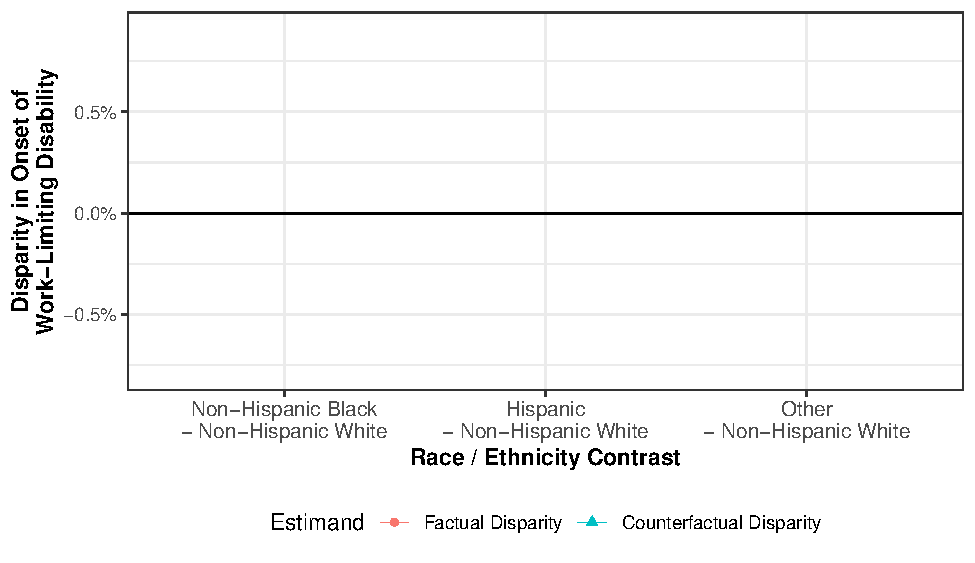
\includegraphics[width = \textwidth]{figures/disparity_1}};
    %\node<2>[anchor = west] at (0,0) {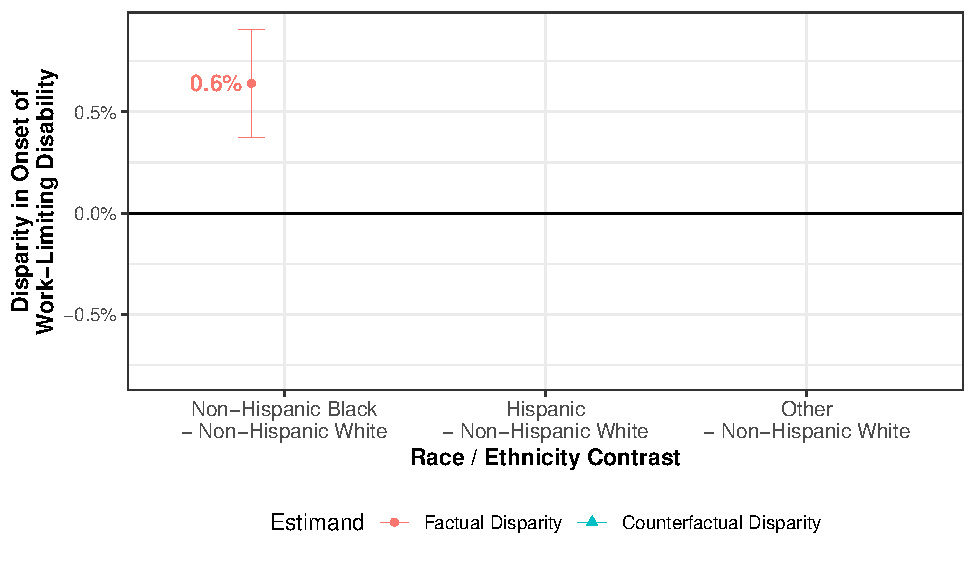
\includegraphics[width = \textwidth]{figures/disparity_2}};
    %\node<3-5>[anchor = west] at (0,0) {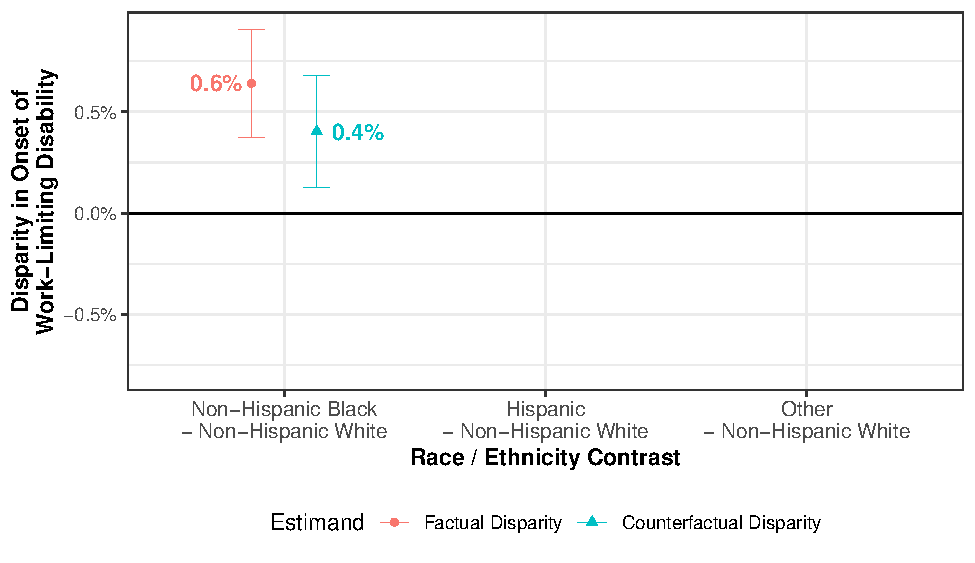
\includegraphics[width = \textwidth]{figures/disparity_3}};
    %\node<6>[anchor = west] at (0,0) {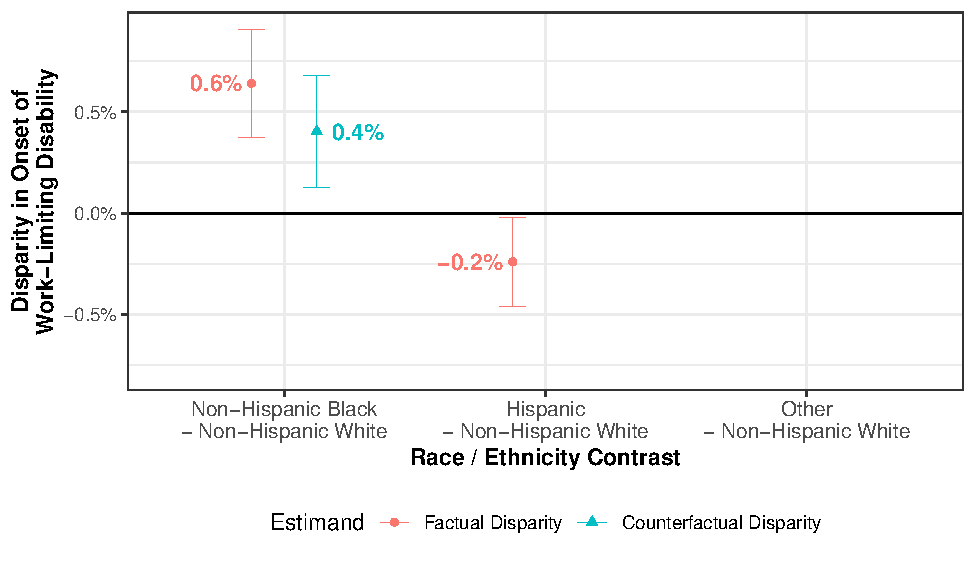
\includegraphics[width = \textwidth]{figures/disparity_4}};
    %\node<7-8>[anchor = west] at (0,0) {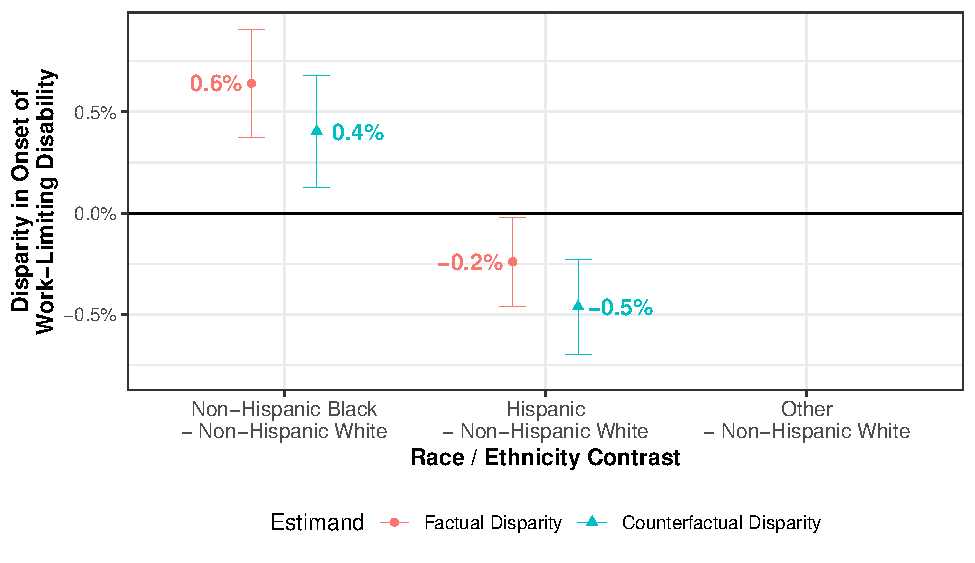
\includegraphics[width = \textwidth]{figures/disparity_5}};
    %\node<9>[anchor = west] at (0,0) {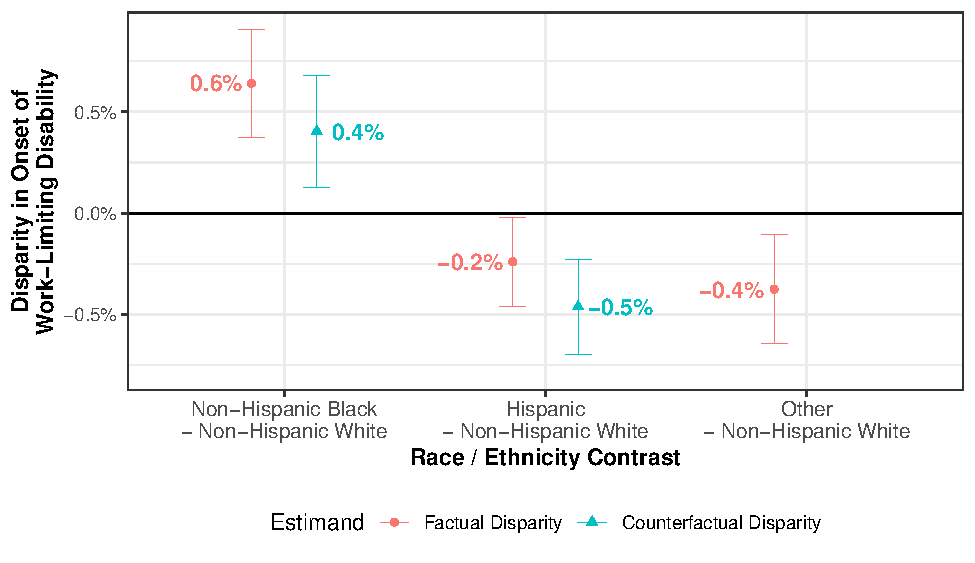
\includegraphics[width = \textwidth]{figures/disparity_6}};
    \node[anchor = north] at (1,4.5) {};
    \node[anchor = west] (figure) at (0,0) {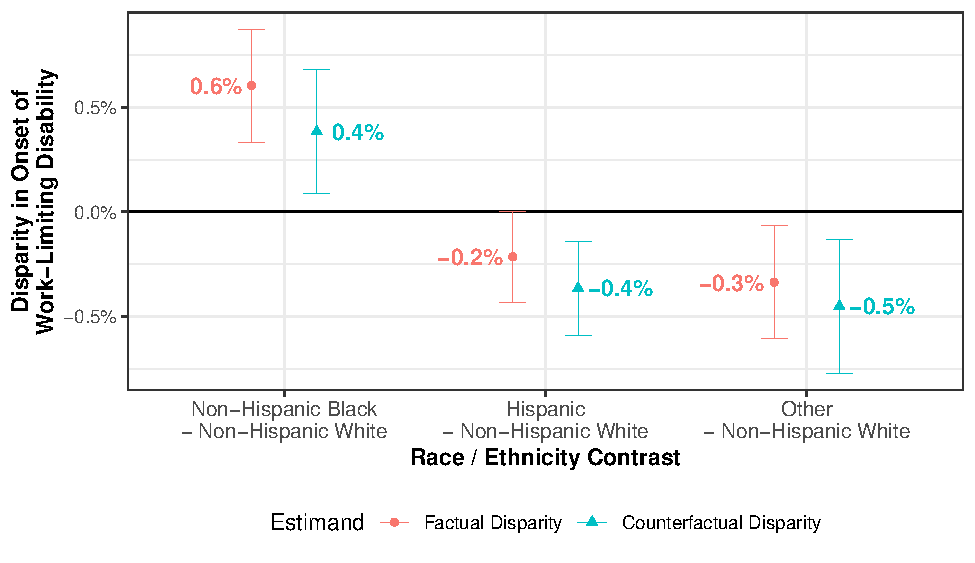
\includegraphics[width = \textwidth]{figures/disparity}};
    \node<2->[anchor = north west] at (0,4.5) {\bgray{Counterfactual:} Assign occupation as a function of education alone};
    % Cover things up
    \draw<1-2>[draw = white, fill = white] (.32,.8) rectangle (.43,2.5);
    \draw<1-4>[draw = white, fill = white] (.58,-1.1) rectangle (.7,.6);
    \draw<1-5>[draw = white, fill = white] (.85,-1.1) rectangle (.97,.6);
    \node<4->[darkgray, font =  \scriptsize] at (.3,0) {36\% reduction};
    \draw<4->[->, thick, darkgray] (.3,.2) to[bend left] (.3, 1.1);
    \node<5->[darkgray, font =  \scriptsize, align = center] at (.57,1.7) {70\% increase\\in magnitude};
    \draw<5->[->, thick, darkgray] (.57,1.2) to[bend left] (.6, .5);
    \node<6->[darkgray, font =  \scriptsize, align = center] at (.85,1.7) {34\% increase\\in magnitude};
    \draw<6->[->, thick, darkgray] (.85,1.2) to[bend left] (.88, .5);
\end{tikzpicture}
\end{frame}

% Plain white frame to mark start of big picture
\begin{frame}
\end{frame}

\section{Big Picture}

% NEW RACE FRAME
\begin{frame}
\begin{tikzpicture}[x = \textwidth, y = \textheight]
\node at (0,0)  {};
\node at (1,1) {};
\node<1->[anchor = west, align = left] (bigPicture) at (0,.9) {\bgray{Big picture}};
\node<1->[anchor = north west, align = left] at (bigPicture.north east) {Counterfactual causal inference can help us\\answer new questions about racial disparities};
\node<2-6>[rotate = 0] at (.5,.5) {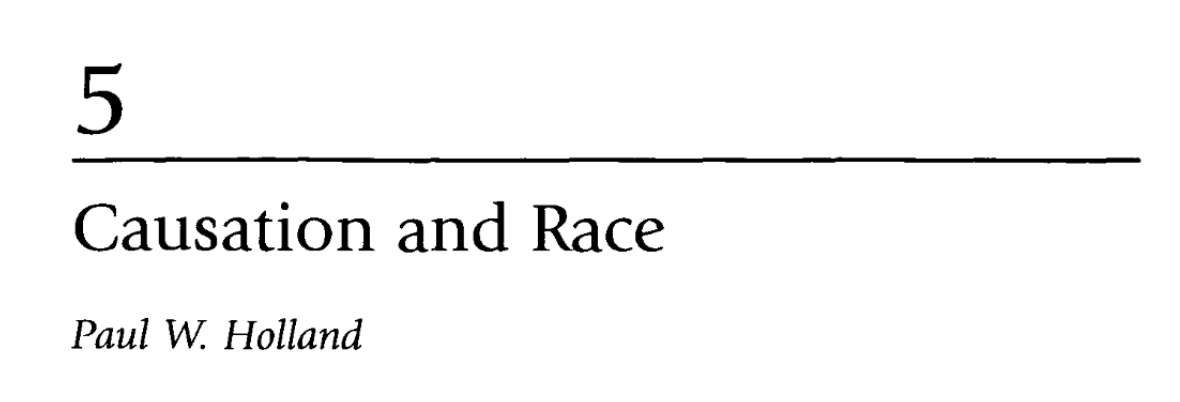
\includegraphics[width = .8\textwidth]{figures/holland_p1}};
\node<3-6>[rotate = 10] at (.5,.5) {
\includegraphics[width = .95\textwidth]{figures/greinerrubin_p1}};
\node<4-6>[rotate = 0] at (.5,.5) {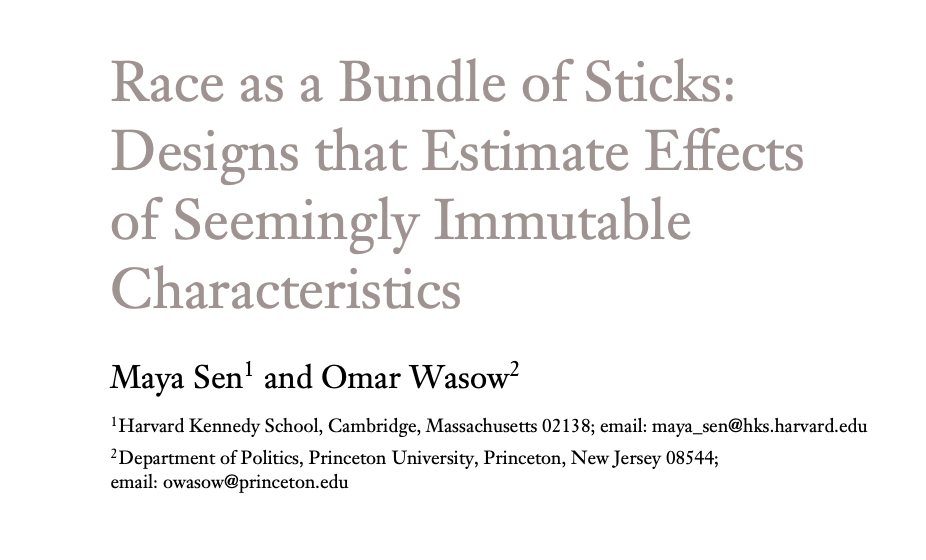
\includegraphics[width = .6\textwidth]{figures/senwasow_p1}};
\node<5-6>[rotate = -10] at (.5,.5) {
\includegraphics[width = .8\textwidth]{figures/bertrandmullainathan_p1}};
\node<6>[rotate = 5] at (.5,.5) {
\includegraphics[width = .8\textwidth]{figures/kohlerhausmann_p1}};
% Begin science table
\node<7>[anchor = north west] at (.05,.77) {
\scalebox{.7}{\begin{tikzpicture}[x = .9in, y = .3in, every node/.style={anchor = center}]
\node at (-1,-4) {};
\node at (0,2) {};
\node[anchor = south, align = center, font = \bf, gray, rotate = 90] at (-.5,-3.5) {Population};
\node at (0,-1) {Person 1};
\node at (0,-2) {Person 2};
\node at (0,-3) {Person 3};
\node at (0,-4) {Person 4};
\node at (0,-5) {Person 5};
\node at (0,-6) {Person 6};
\node[font = \bf, gray] at (1.5,1) {Treatment Condition};
\node at (1,0) {Black};
\node at (2,0) {White};
\draw[thick] (.6,-.5) -- (1.4,-.5);
\draw[thick] (1.6,-.5) -- (2.4,-.5);
\node at (1,-1) {$Y_1(\text{Black})$};
\node at (2,-1) {$Y_1(\text{White})$};
\node at (1,-2) {$Y_2(\text{Black})$};
\node at (2,-2) {$Y_2(\text{White})$};
\node at (1,-3) {$Y_3(\text{Black})$};
\node at (2,-3) {$Y_3(\text{White})$};
\node at (1,-4) {$Y_4(\text{Black})$};
\node at (2,-4) {$Y_4(\text{White})$};
\node at (1,-5) {$Y_5(\text{Black})$};
\node at (2,-5) {$Y_5(\text{White})$};
\node at (1,-6) {$Y_6(\text{Black})$};
\node at (2,-6) {$Y_6(\text{White})$};
\end{tikzpicture}}
};
\node<8->[anchor = north west] at (.05,.77) {
\scalebox{.7}{\begin{tikzpicture}[x = .9in, y = .3in, every node/.style={anchor = center}]
\node at (-1,-4) {};
\node at (0,2) {};
\node<8->[anchor = south, align = center, font = \bf, gray, rotate = 90] at (-.5,-2) {Black};
\node<8->[anchor = south, align = center, font = \bf, gray, rotate = 90] at (-.5,-5.5) {White};
\draw[line width = 1.2pt, gray] (-.45,-.7) -- (-.45,-3.3);
\draw[line width = 1.2pt, gray] (-.45,-4.2) -- (-.45,-6.8);
\node at (0,-1) {Person 1};
\node at (0,-2) {Person 2};
\node at (0,-3) {Person 3};
\node at (0,-4.5) {Person 4};
\node at (0,-5.5) {Person 5};
\node at (0,-6.5) {Person 6};
\only<9->{
\node[align = center] at (1,.4) {As\\observed};
\draw[thick] (.6,-.3) -- (1.4,-.3);
\node at (1,-1) {$Y_1$};
\node at (1,-2) {$Y_2$};
\node at (1,-3) {$Y_3$};
\node at (1,-4.5) {$Y_4$};
\node at (1,-5.5) {$Y_5$};
\node at (1,-6.5) {$Y_6$};
}
\only<10->{
\draw[draw = white, fill = gray, fill opacity = .2, rounded corners] (.7,-3.5) rectangle (1.3, -.5);
\draw[draw = white, fill = gray, fill opacity = .2, rounded corners] (.7,-7) rectangle (1.3, -4);
\node[anchor = north, font = \bf, gray, align = center] at (1,-7.3) {Descriptive\\Disparity};
}
\only<12->{
\draw[draw = white, fill = blue, fill opacity = .2, rounded corners] (1.7,-3.5) rectangle (2.3, -.5);
\draw[draw = white, fill = blue, fill opacity = .2, rounded corners] (1.7,-7) rectangle (2.3, -4);
\node<15->[anchor = north, font = \bf, blue, align = center, opacity = .5] at (2,-7.3) {Gap-Closing\\Estimand};
}
\only<11->{
\node[align = center] at (2,.4) {Under\\intervention};
\draw[thick] (1.6,-.3) -- (2.4,-.3);
\node at (2,-1) {$Y_1(t)$};
\node at (2,-2) {$Y_2(t)$};
\node at (2,-3) {$Y_3(t)$};
\node at (2,-4.5) {$Y_4(t)$};
\node at (2,-5.5) {$Y_5(t)$};
\node at (2,-6.5) {$Y_6(t)$};
}
\end{tikzpicture}}
};
\draw<13->[line width = 1pt, line cap = round, blue, draw opacity = .5] (.33,.825) -- (.54,.825);
\draw<14->[->, line width = 1pt, line cap = round, blue, draw opacity = .5] (.445,.81) to[bend right] (.73,.7);
\node<14->[anchor = east, font = \footnotesize, align = center, draw = blue, draw opacity = .5, rounded corners, line width = 1pt] at (1,.7) {How much would\\the gap close\\if we intervene?};
\node<15->[anchor = south east, font = \scriptsize, align = left, gray] (c3) at (1,.15) {Lundberg 2021};
\only<16->{
\node[anchor = south east, font = \scriptsize, align = left, gray] (c2) at (c3.north east) {Jackson \& Vanderweele 2018};
\node[anchor = south east, font = \scriptsize, align = left, gray] (c1) at (c2.north east) {Vanderweele \& Robinson 2014};
}
\end{tikzpicture}
\end{frame}

\begin{frame}
\begin{center}
%Quantifying the contribution of occupational segregation\\to racial disparities in health:\\
%A gap-closing perspective \vskip .3in
Ian Lundberg\\
ianlundberg@ucla.edu
\vskip .5in
\begin{small}
\begin{tabular}{rl}
Paper on SocArXiV & \href{https://doi.org/10.31235/osf.io/x9evk}{\textcolor{blue}{osf.io/x9evk/}} \\
Code on GitHub & \href{https://github.com/ilundberg/replication/tree/master/occupational_segregation_health}{\textcolor{blue}{github.com/ilundberg/replication}}
\end{tabular}
\end{small}
\end{center} 
\end{frame}

\end{document}

% BARS + SCATTERS
\begin{frame}
\label{descriptive_results}
\begin{tikzpicture}[x = \textwidth, y = \textheight]
\node at (0,0) {};
\node at (1,1) {};
\node<1->[anchor = north east, font = \footnotesize, align = right, gray] (note1) at (1,.65) {Current\\Population Survey\\Annual Social and\\Economic Supplement\\Ages 25--60\\2005--2020};
\node<2->[anchor = south west, align = left, text width = .87\textwidth, font = \footnotesize, fill = lightgray, fill opacity = .4, text opacity = 1, rounded corners] at (0,.8) {Do you have a health problem or disability which prevents you from working or which limits the kind or amount of work you can do?};
\node<3>[anchor = north west] at (0,.7) {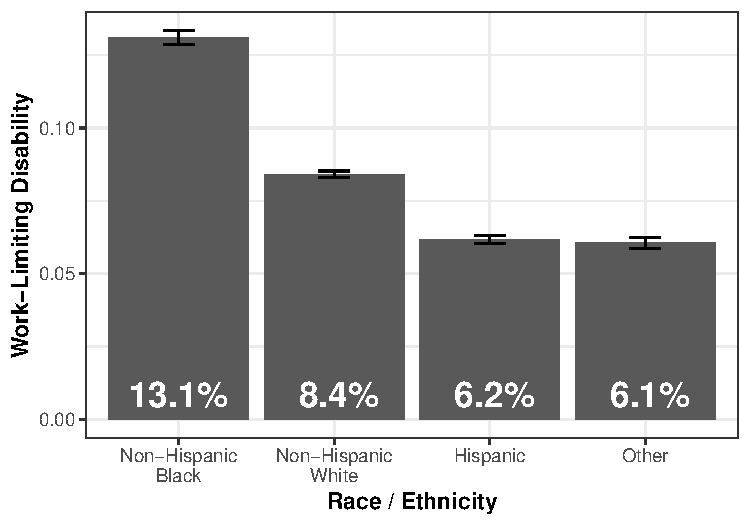
\includegraphics[width = .68\textwidth]{figures/disability_by_race}};
% Timeline
\draw<4-6>[->, gray, line width = 2pt] (0,.5) -- (.65, .5);
\draw<4-6>[thick] (.15,.48) -- (.15, .52);
\draw<4-6>[thick] (.5,.48) -- (.5, .52);
\node<4-6>[anchor = south, font = \footnotesize] at (.15,.52) {Year $y$};
\node<4-6>[anchor = south, font = \footnotesize] at (.5,.52) {Year $y + 1$};
\node<5-6>[anchor = north, font = \footnotesize, align = center] at (.15,.48) {\bgray{Restriction}\\Employed with\\no work-limiting\\disability};
\node<6>[anchor = north, font = \footnotesize, align = center] at (.5,.48) {\bgray{Outcome}\\Onset of\\work-limiting\\disability};
% Onset results
\node<7>[anchor = north west] at (0,.7) {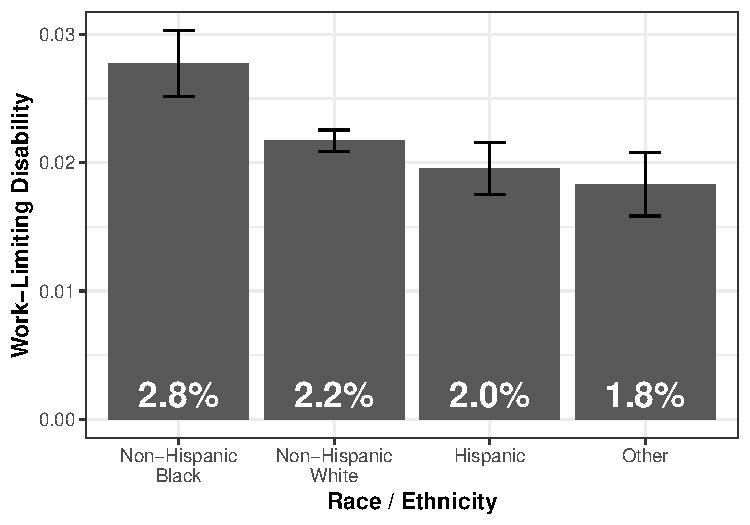
\includegraphics[width = .68\textwidth]{figures/onset_by_race}};
\node<7->[anchor = north east, font = \footnotesize, align = right, gray] at (note1.south east) {Employed last year\\No disability\\last year};
\node<7>[anchor = south west, align = left] at (.1,.7) {\textbf{Onset of Work-Limiting Disability}};
\node<8>[anchor = north west] at (0,.7) {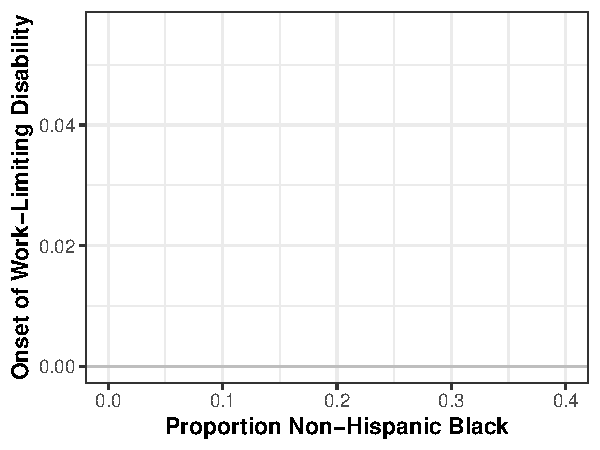
\includegraphics[width = .68\textwidth]{figures/scatter_factual_outcome_re_NonHispanicBlack_slide1}};
\node<9>[anchor = north west] at (0,.7) {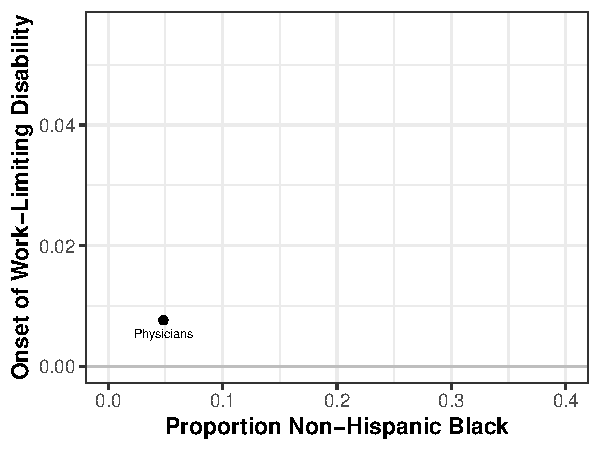
\includegraphics[width = .68\textwidth]{figures/scatter_factual_outcome_re_NonHispanicBlack_slide2}};
\node<10>[anchor = north west] at (0,.7) {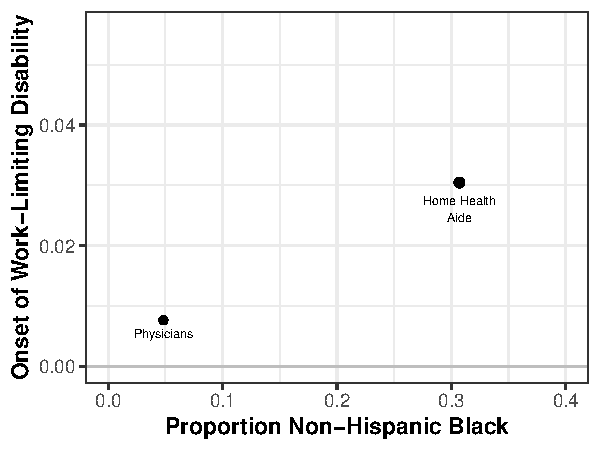
\includegraphics[width = .68\textwidth]{figures/scatter_factual_outcome_re_NonHispanicBlack_slide3}};
\node<11>[anchor = north west] at (0,.7) {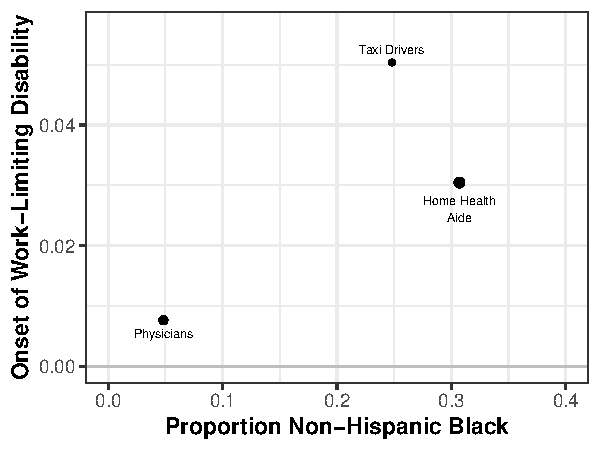
\includegraphics[width = .68\textwidth]{figures/scatter_factual_outcome_re_NonHispanicBlack_slide4}};
\node<12>[anchor = north west] at (0,.7) {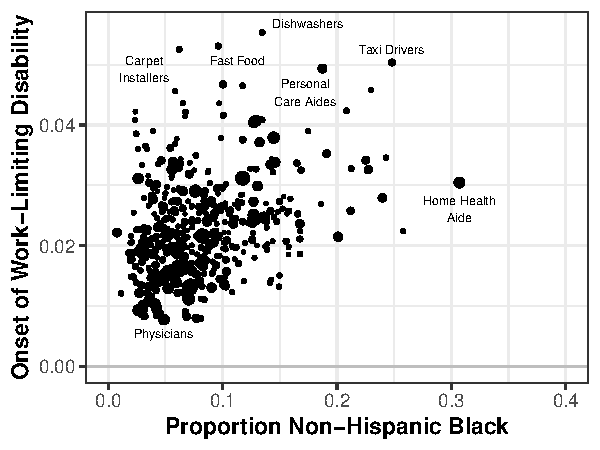
\includegraphics[width = .68\textwidth]{figures/scatter_factual_outcome_re_NonHispanicBlack_slide5}};
\node<13>[anchor = north west] at (0,.7) {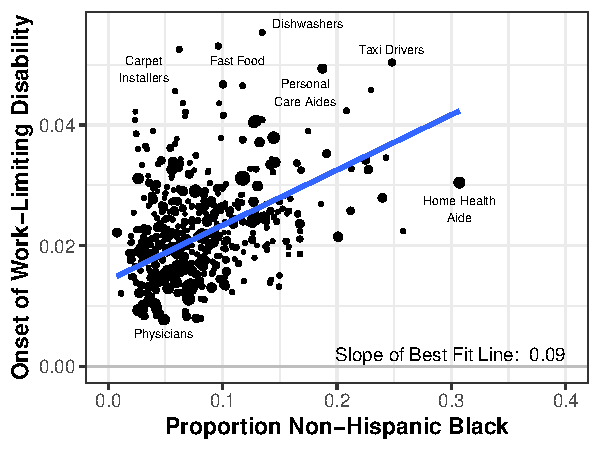
\includegraphics[width = .68\textwidth]{figures/scatter_factual_outcome_re_NonHispanicBlack_slide6}};
%\node<14->[anchor = north west] at (0,.7) {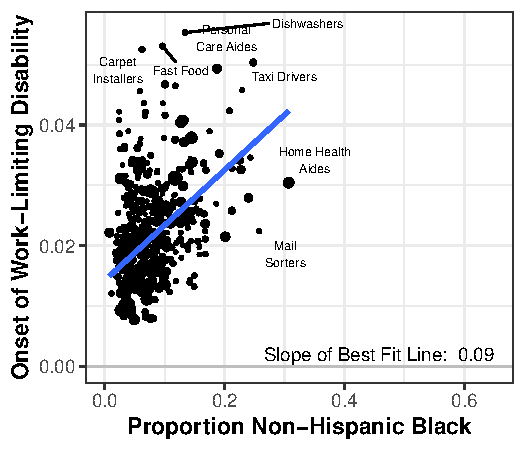
\includegraphics[width = .3\textwidth]{figures/scatter_factual_outcome_re_NonHispanicBlack_annotated}};
%\node<15->[anchor = north west] at (0,.4) {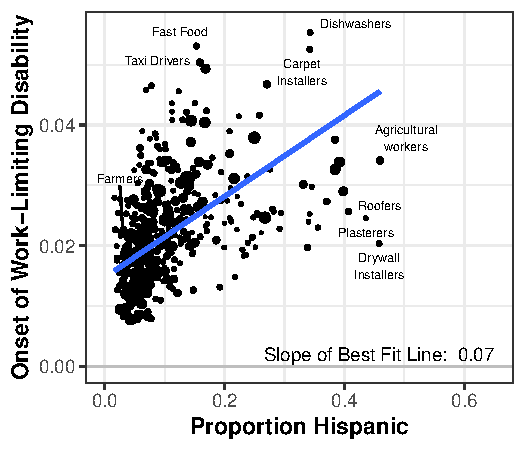
\includegraphics[width = .3\textwidth]{figures/scatter_factual_outcome_re_Hispanic_annotated}};
%\node<16->[anchor = north west] at (.35,.7) {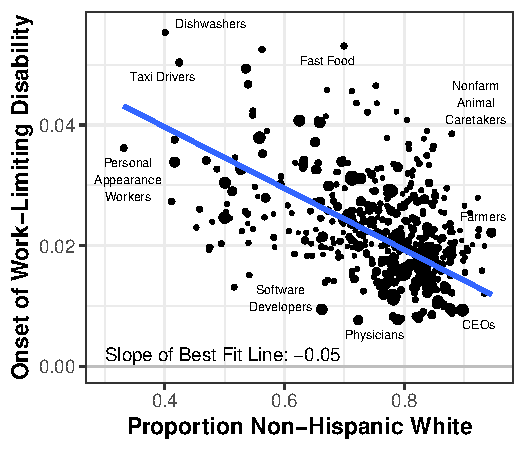
\includegraphics[width = .3\textwidth]{figures/scatter_factual_outcome_re_NonHispanicWhite_annotated}};
%\node<17->[anchor = north west] at (.35,.4) {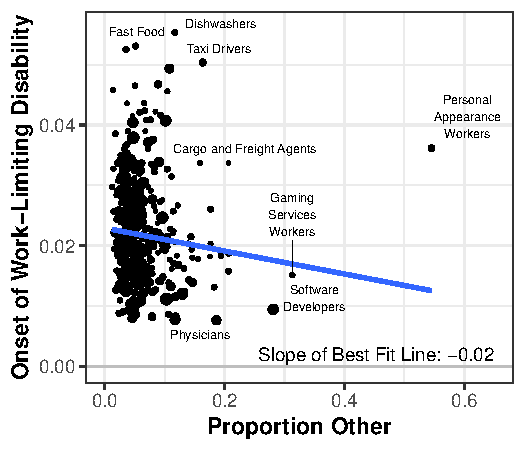
\includegraphics[width = .3\textwidth]{figures/scatter_factual_outcome_re_Other_annotated}};
%\node<18>[anchor = south west, align = left] at (0,.8) {To what degree does \bblue{occupational segregation}\\contribute to \bblue{racial health disparities}?};
\end{tikzpicture}
\end{frame}




